% !TeX root = main.tex

% ============================================================
% thesis-sync entry: 2026-07-06_leg-actuator-suction-foot
% Type: design decision + numeric data
% Insertable section block (no preamble). Requires: graphicx.
% Figure \includegraphics lines are COMMENTED so the file compiles standalone.
% ============================================================

\section{LEG ACTUATORS AND SUCTION-CUP FEET}
\label{sec:lizard-legs}

\subsection{Leg Actuator Design}

Each of the four legs is a single-chambered fiber-reinforced bending
actuator, structurally simpler than the three-chambered body--tail
segments: a leg needs to bend only in one plane (lifting and planting the
foot), so omnidirectionality is unnecessary and a single chamber
minimizes the pneumatic channel count. The silicone tube is 24~mm long
(30~mm overall actuator length including the end interfaces) and is
reinforced by a double-helical fiber winding with an average pitch angle
of 20$^{\circ}$, which constrains radial expansion while permitting axial
strain \cite{Mao2020Soft}. A single additional fiber is placed
longitudinally along one side of the tube. This longitudinal fiber acts
as an inextensible constraint layer: under pressurization, the
constrained side cannot elongate while the free side does, so the
actuator bends toward the fiber side. In the robot experiments, the leg
actuators reach a bending angle of approximately 90$^{\circ}$ at an input
pressure of 13~kPa.

\subsection{Suction-Cup Feet}

Each leg terminates in a suction-cup foot cast in Elastosil M4601, with
an outer diameter of 10~mm and an internal vacuum height of 3~mm. The
cups are actively evacuated: a dedicated vacuum line, supplied by the
same multichannel pneumatic system that drives the positive-pressure
channels, is switched to attach and release each foot. Each leg therefore
carries two pneumatic ports, a positive-pressure port for the bending
chamber and a vacuum port for the foot. Active evacuation allows
attachment and release to be commanded at specific phases of the gait,
which passive suction cups do not permit.

% --- Figures (paths to be fixed by the author; commented for compilation) ---
\begin{figure}[tb]
  \centering
  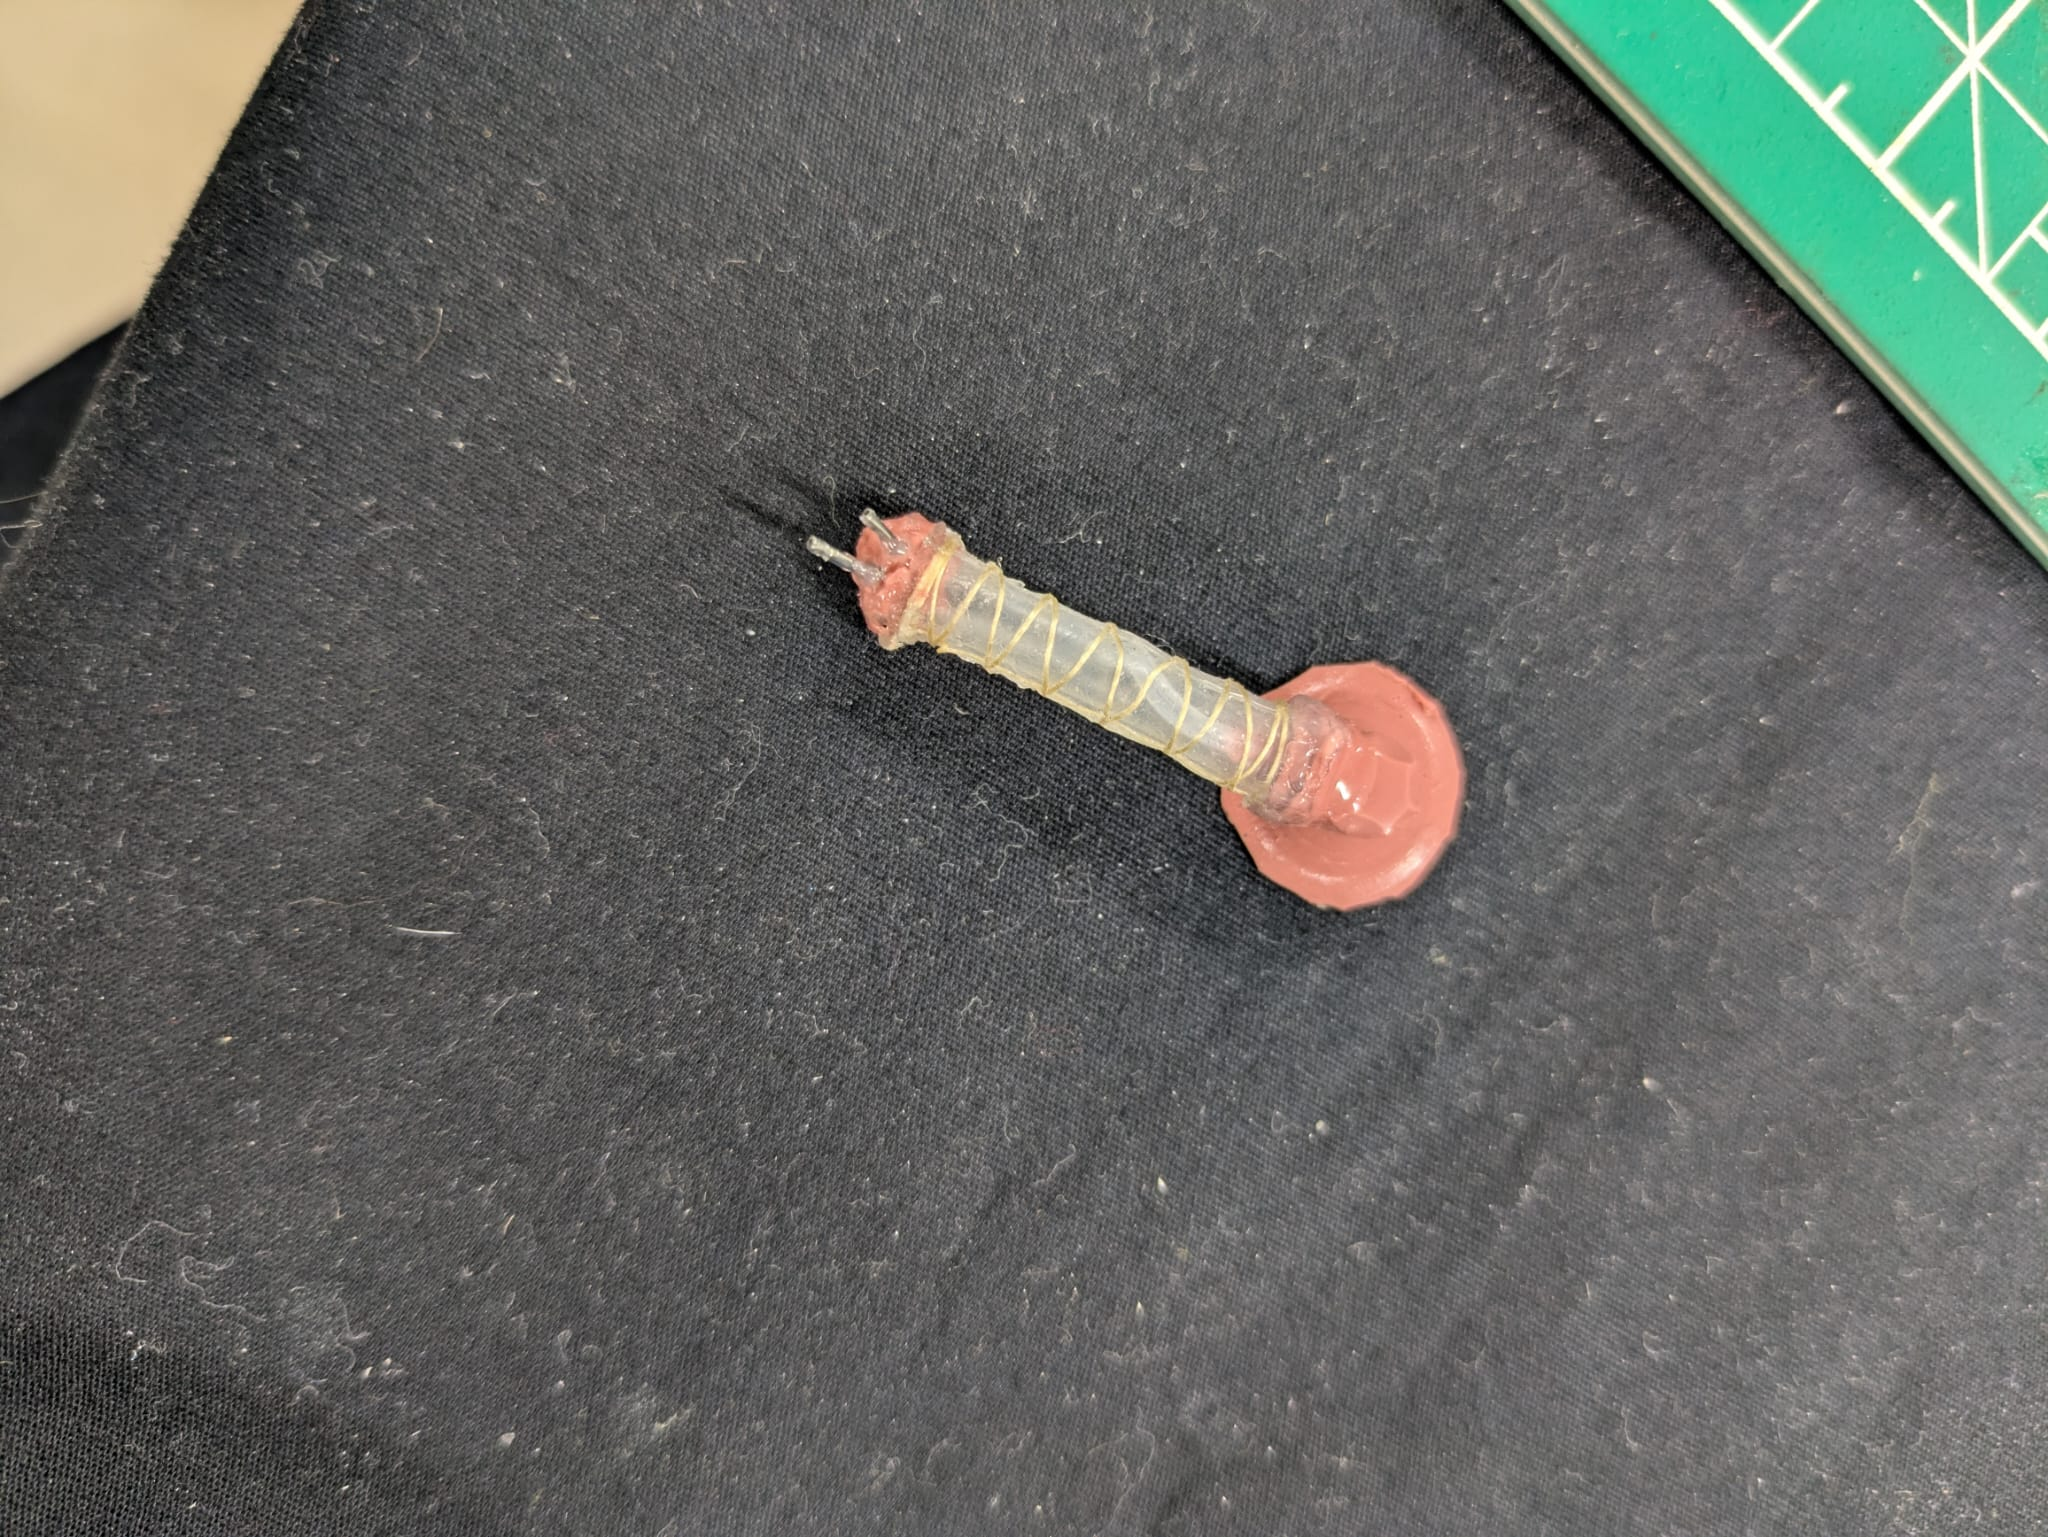
\includegraphics[width=0.8\columnwidth]{figures/lizardleg.jpeg}
  \caption{Single leg actuator prior to integration. The double-helical
  fiber winding is visible on the 24~mm silicone tube; the Elastosil
  M4601 suction-cup foot (10~mm outer diameter) is cast onto the distal
  end, and the two pneumatic ports (positive pressure for the bending
  chamber, vacuum for the cup) protrude from the proximal end cap.}
  \label{fig:lizard-leg}
\end{figure}
